%; whizzy chapter
% -initex iniptex -latex platex -format platex -bibtex jbibtex -fmt fmt
% 以上 whizzytex を使用する場合の設定.

%     Kansai Debian Meeting resources
%     Copyright (C) 2007 Takaya Yamashita
%     Thank you for Tokyo Debian Meeting resources

%     This program is free software; you can redistribute it and/or modify
%     it under the terms of the GNU General Public License as published by
%     the Free Software Foundation; either version 2 of the License, or
%     (at your option) any later version.

%     This program is distributed in the hope that it will be useful,
%     but WITHOUT ANY WARRANTY; without even the implied warranty of
%     MERCHANTABILITY or FITNESS FOR A PARTICULAR PURPOSE.  See the
%     GNU General Public License for more details.

%     You should have received a copy of the GNU General Public License
%     along with this program; if not, write to the Free Software
%     Foundation, Inc., 51 Franklin St, Fifth Floor, Boston, MA  02110-1301 USA

%  preview (shell-command (concat "evince " (replace-regexp-in-string "tex$" "pdf"(buffer-file-name)) "&"))
% 画像ファイルを処理するためには ebb を利用して boundingbox を作成.
%(shell-command "cd image200708; ebb *.png")

%%ここからヘッダ開始.

\documentclass[mingoth,a4paper]{jsarticle}
\usepackage{kansaimonthlyreport}
\usepackage[dvips]{xy}
\usepackage{ascmac}

% 日付を定義する, 毎月変わります.
\newcommand{\debmtgyear}{2011}
\newcommand{\debmtgmonth}{10}
\newcommand{\debmtgdate}{23}
\newcommand{\debmtgnumber}{52}

\begin{document}

\begin{titlepage}

% 毎月変更する部分, 本文の末尾も修正することをわすれずに

 第\debmtgnumber{}回 関西 Debian 勉強会資料

\vspace{2cm}

\begin{center}
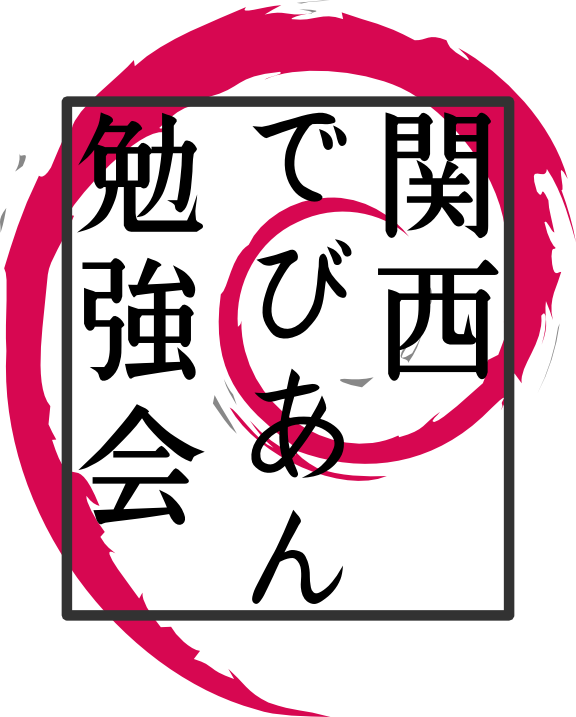
\includegraphics{image200802/kansaidebianlogo.png}
\end{center}

\begin{flushright}
\hfill{}関西 Debian 勉強会担当者 佐々木・倉敷・のがた \\
\hfill{}\debmtgyear{}年\debmtgmonth{}月\debmtgdate{}日
\end{flushright}

\thispagestyle{empty}
\end{titlepage}

\dancersection{Introduction}{Debian JP}

\subsection*{}%ロゴ用のスペース稼ぎ

関西 Debian 勉強会は Debian GNU/Linux のさまざまなトピック (新しいパッケー
ジ, Debian 特有の機能の仕組, Debian 界隈で起こった出来事, などなど) に
ついて話し合う会です.

目的として次の三つを考えています.
\begin{itemize}
      \item ML や掲示板ではなく, 直接顔を合わせる事での情報交換の促進
      \item 定期的に集まれる場所
      \item 資料の作成
\end{itemize}

それでは, 楽しい一時をお楽しみ下さい.

\clearpage

\begin{minipage}[b]{0.2\hsize}
 {\rotatebox{90}{\fontsize{80}{80}
{\gt 関西 Debian 勉強会}}}
\end{minipage}
\begin{minipage}[b]{0.8\hsize}
\hrule
\vspace{2mm}
\hrule
\setcounter{tocdepth}{1}
\tableofcontents
\vspace{2mm}
\hrule
\end{minipage}


\dancersection{最近の Debian 関係のイベント報告}{Debian JP}

\subsection{第 51 回関西 Debian 勉強会}
51 回目の関西 Debian 勉強会は 2011 年 9 月 25 日(日)に福島区民センターで
開催されました。

\subsection{第 81 回東京エリア Debian 勉強会 @ 筑波大学}
81回目の東京エリアDebian勉強会は、筑波大学にて、つくらぐ(筑波大学 Linux
User Group)と合同でおこなわれたそうです。


\clearpage
%-------------------------------------------------------------------------------
\dancersection{事前課題}{Debian JP}

今回は以下の事前課題を設定しました。


\begin{enumerate}
 \item EmacsもしくはVimの拡張機能のDebianパッケージを挙げてください(何個でも)。また、それらに含まれるファイル一覧を見ておいてください(これは記入不要)
 \item OmegaT が動作する環境1を用意し, お手軽スタートガイドに目を通してきて下さい。翻訳をしたことがある人は作業環境を教えて下さい。
\end{enumerate}

参加者の皆さんによる回答は以下の通りです。

\begin{prework}{ kozo2 }
  \begin{enumerate}
  \item Emacs: auto-install-el, twittering-mode, auto-complete-el, anything-el\\
    Vim: vim-rails
  \item Sphinx
  \end{enumerate}
\end{prework}

\begin{prework}{ Y.YATSUO }
  \begin{enumerate}
  \item vim-scripts ... vim にベルとホイッスル機能を追加するプラグイン \\
    こんなのあるんですね…
  \item ちょっとした文章なら vim で翻訳します.
  \end{enumerate}
\end{prework}

\begin{prework}{ 川江 }
  \begin{enumerate}
  \item 拡張機能は使った事がないので勉強しておきます。
  \item 見ておきます。
  \end{enumerate}
\end{prework}

\begin{prework}{ gdevmjc }
  \begin{enumerate}
  \item egg c-sig mew-beta
  \item とりあえず、 squeeze の omegat 1.8.1 を入れましたa
  \end{enumerate}
\end{prework}

\begin{prework}{ かわだてつたろう }
 \begin{enumerate}
  \item apel, flim, semi, auto-install-el, ddskk, easypg, elscreen, howm,
        lookup-el, sdic, wl-beta
  \item 用意して目を通しました。 
 \end{enumerate}
\end{prework}

\begin{prework}{ のがたじゅん }
 \begin{enumerate}
  \item psgml, css-mode, org-mode, gettext-el, muse-el, yatex
  \item 翻訳するときgettextのファイルが多いので、emacs上のgettext-elを使っています。
 \end{enumerate}
\end{prework}

\begin{prework}{ shuttaholic }
 \begin{enumerate}
  \item vim-syntax-go, vim-puppet, supercollider-vim, vim-athena,
        vim-dbg, vim-lesstif, vim-addon-manager, vim-latexsuite,
        vim-rails, vim-syntax-gtk, vimhelp-de, vim-vimoutliner,
        vim-scripts
 \end{enumerate}
\end{prework}

\begin{prework}{ 松澤二郎 }
 \begin{enumerate}
  \item vim-scripts
  \item Debianの翻訳に携わったことはなく、GNOMEプロジェクトでの作業になり
        ますが、PO編集が作業の中心で、テキストエディター(vim, geditなど)
        とtranslate-toolkitで作業することが多いです。バージョン管理には
        gitを使っています。OmegaTは私にはちょっと難しくて疎遠になっていま
        したが、これを機にがんばって覚えたいと思います。
 \end{enumerate}
\end{prework}

\begin{prework}{ よしだともひろ }
 \begin{enumerate}
  \item Emacs: mew, howm, twittering-mode, autocompleteなど \\
        Vim: すみません、よくわかりません
  \item OmegaT バージョン2.3.0 アップデート1をインストールしました。
        お手軽スタートガイドを読みました。
 \end{enumerate}
\end{prework}

\begin{prework}{ lurdan }
 \begin{enumerate}
  \item ddskk, org-mode, howm, ack-grep, lookup-el, anything-el,
        autoinstall-el, auto-complete-el, emacs-calfw, apel, flim, semi,
        wl-beta, riece, w3m-el, puppet-el, vim-puppet
  \item emacs + skk + lookup-el + po-mode
 \end{enumerate}
\end{prework}


\clearpage
%------------------------------------------------------------------------------
\dancersection{Emacs, Vim の拡張機能で学ぶ Debian パッケージ}{西田孝三}

\subsection{はじめに}

パッケージメンテナになることでDebianに関わりたいと思われている方は多いのではないでしょうか。
もしあなたがEmacs, Vimのユーザであればこれらの機能拡張でパッケージを作成するところから始めて
みるのはどうでしょうか。
理由は、
\begin{itemize}
 \item アーキテクチャに依存しない
 \item コンパイルは不要 (Emacsの場合バイトコンパイルがありますが)
\end{itemize}
などから比較的簡単と思われるためです。

ここでは大きく分けて下記のことを行い、まずは簡単なDebianパッケージを自分で作成できるようにな
るまでを目的としています。

\begin{itemize}
  \item EmacsのDebianパッケージ
    \begin{itemize}
      \item 既存のDebianパッケージの構成を知り再構成を行う
      \item 独自のDebianパッケージを作成する
    \end{itemize}
  \item VimのDebianパッケージ
    \begin{itemize}
      \item 既存のDebianパッケージの構成を知る
    \end{itemize}
\end{itemize}

Vimでは構成だけを学び、独自のDebianパッケージの作成を行いません。その理由は後に説明します。
それではEmacsの既存のDebianパッケージの構成を知り再構成を行うところから始めましょう。

\subsection{EmacsのDebianパッケージ}

\subsubsection{Emacsの既存Debianパッケージのソース取得と再構成}

ここでは前回の関西Debian勉強会で発表されていた山下尊也さんがメンテナンスをされている
auto-install-elのパッケージのソースを取得し、再構成を行います。

\begin{commandline}
 $ mkdir tmp; cd tmp
 $ apt-get source auto-install-el
 $ ls auto-install-el-1.48
\end{commandline}

これでtmpディレクトリ内にauto-install-elのソース(バージョン1.48)が取得できているはずです。
ソース内容を確認することは保留し、いきなりDebianパッケージを作ってみましょう。

\begin{commandline}
 $ cd auto-install-el-1.48
 $ debuild -us -uc
 $ ls ..
\end{commandline}

これでdebuildをしたディレクトリのひとつ上にauto-installのDebianパッケージができます。
それではこのDebianパッケージをインストールしてみましょう。

\begin{commandline}
 $ cd ..
 $ sudo dpkg -i auto-instlal-el_1.48-1_all.deb
 $ aptitude show auto-install-el
\end{commandline}

これでauto-install-elがインストールされたことがわかります。
それではうまく使えるかどうかEmacsで確認してみましょう。

\begin{commandline}
 $ emacs -nw
 M-x load-library
 auto-install
 auto-install-from-emacswiki
 grep-edit.el
\end{commandline}

これで ~/.emacs.d/auto-install/ 下にgrep-edit.el(elc)がインストールされていることが
確認できます。

それでは保留していたソースの構成の確認に戻りましょう。
が、その前にもう一つ別のディレクトリにauto-install-elのソースを取得しましょう。
というのはdebuild後にはいくつかのファイルが生成されているからです。
2つのソースディレクトリを比較することでこれらのファイルが確認できます。
詳細はご自身でご確認ください。

\begin{commandline}
 $ cd; mkdir auto-install-el
 $ cd auto-install-el; apt-get source auto-install-el
\end{commandline}

それではdebuildする前のauto-install-el-1.48内のファイル構成を見てみましょう。
auto-install.elというファイルとdebianというディレクトリがあります。
このことからEmacsの拡張機能のDebianパッケージを作るには

\begin{itemize}
 \item Emacsの拡張機能にバージョン名を加えた名前のディレクトリを作り
 \item その下にEmacs Lispとdebianというディレクトリを作ればよい
\end{itemize}

ということがわかります。それではこれをまだDebianパッケージが作られていないEmacs
の拡張機能に対して行っていきましょう。

\subsubsection{Emacsの新規Debianパッケージの作成}

今回は青田直大さんによるtwinstall.elのパッケージを作ってみましょう。
これはtwittering-modeというEmacs用twitterクライアントの機能を使って、
auto-install.elでインストールしたEmacs Lisp名をつぶやくものです。
現時点ではIDが1300477のgist(https://gist.github.com/1300477)から取得できます。

\begin{commandline}
 $ tar zxvf gist1300477.tar.gz
 $ mv gist1300477 twinstall-el-0.1
 $ tar czvf twinstall-el-0.1.tar.gz twinstall-el-0.1
 $ cd twinstall-el-0.1
 $ cat >>~/.bashrc <<EOF
  DEBEMAIL=''your.email.address@example.org''
  DEBFULLNAME=''Firstname Lastname''
  export DEBEMAIL DEBFULLNAME
  EOF
 $ . ~/.bashrc
 $ dh_make -f ../twinstall-el-0.1.tar.gz
\end{commandline}

次にどのような種類のパッケージを作るか聞かれるのでsingleのsにしenterを押します。
するとdebianディレクトリとその下に各種設定ファイルの雛形が生成されます。
多くのファイルができあがりますが、auto-install-elと同じものがあればよいので対応す
るファイルは削除し、後はauto-install-elを真似てファイル内容を変更していきましょう。
(変更せずにこの段階でdebuildを行っても一応パッケージはできます。)
それでは各ファイルの説明をします。

\clearpage

\paragraph{\texttt{README.Debian}}
  \begin{itemize}
    \item DebianパッケージのREADME
    \item 必須ではない?
  \end{itemize}

\paragraph{\texttt{changelog}}
  \begin{itemize}
    \item 必須のファイル
    \item Debianのポリシーで規定された書式
  \end{itemize}

\paragraph{\texttt{compat}}
  \begin{itemize}
    \item わかりませんでした!
    \item 作られた雛形のままにしましょう
  \end{itemize}

\paragraph{\texttt{control}}
  \begin{itemize}
    \item 必須のファイル
    \item aptitudeなどのパッケージ管理ツールが利用する情報
    \item Debianのポリシーで規定された書式
    \item twinstall.elはauto-installとtwittering-modeに依存している。Depends:に追加
  \end{itemize}

\paragraph{\texttt{copyright}}
  \begin{itemize}
    \item 必須のファイル
    \item upstreamソースに関する著作権やライセンスなどの情報を書く
    \item Debianのポリシーで規定された書式
  \end{itemize}

\paragraph{\texttt{dirs}}
  \begin{itemize}
    \item ファイルをインストールするディレクトリを書く
    \item 前述ディレクトリのパスのトップの/は書かない
  \end{itemize}

\paragraph{\texttt{emacsen-install, emacsen-remove}}
  \begin{itemize}
    \item install, uninstall時に行う処理をやってくれるシェルスクリプト
  \end{itemize}

\paragraph{\texttt{emacsen-startup}}
  \begin{itemize}
    \item elispのインストールディレクトリにdirsで書いたインストール先をEmacsのload-pathに追加してくれるelisp
    \item これ自体は/etc/emacs/site-start.d/に50'パッケージ名'.elという名でインストールされる
  \end{itemize}

\paragraph{\texttt{rules}}
  \begin{itemize}
    \item 必須のファイル
    \item パッケージを作成するために使うルールを書く
    \item まずはとりあえず人様のものを真似る
  \end{itemize}

\paragraph{\texttt{source}}
  \begin{itemize}
    \item わかりませんでした!
    \item 作られた雛形のままにしましょう
  \end{itemize}

\begin{commandline}
 $ debuild -us -uc
 $ cd ..
 $ sudo dpkg -i twinstall-el_0.1-1_all.deb
\end{commandline}

controlのDepends以外はauto-install-elを真似て新規パッケージに応じた情報に置き換えることでtwinstallのDebianパッケージが出来ます。
後はこのDebianパッケージを公開する必要があるかを考え、ライセンスなどを学び、公開に必要な次のステップへ進んでください。
もちろんコンパイルが必要なパッケージ作成へとレベルアップするのもよいでしょう。

\subsection{Vimの既存パッケージのソース取得}

Vimの拡張機能のDebianパッケージはEmacsと比較すると数は少なく、あまりパッケージを作るモチベーションが得られなさそうです。
そのためVimに関してはパッケージ作成までは行いません。
実際にRails用のVim scriptパッケージのソースを取得しその内容をみてみましょう。

\begin{commandline}
 $ apt-get source vim-rails
\end{commandline}

これで取得できるソースのREADME.Debianとcontrolを見るとvim-addon-managerというパッケージを使いvim-addonsというコマンドで
vim-railsを使用可能にするということを行なっていることがわかります。
これではDebianのパッケージマネージャーとVimのaddon-managerでmanagerを2つ用いていることになり、あまり良いこととは思えません。
現在のVimユーザの多くはvim-addon-managerよりbundleやneobundleといったVim scriptで書かれたmanagerを用いており、これらの完成
度が高いためDebianのパッケージは不要なのかもしれません。


%$
\clearpage
%------------------------------------------------------------------------------
\dancersection{翻訳で Debian に貢献しよう}{八津尾 雄介}

\subsection{はじめに}
Debian を利用する以上, 英語との付き合いは避けて通れない問題だと思います. 英語の
文章を読むのが苦にならない人から, エラーメッセージさえ読む努力を放棄する人まで, 
様々だとは思いますが, もっと英語ができればと思う事が誰でも少なからずあると思い
ます.

私は英語と付き合う第一歩として, 翻訳をおすすめします. 翻訳というと特殊技術だとか自
分には無理と身構えてしまう人も多いかもしれませんが, それほど敷居の高い作業ではあ
りません.

辞書と基本文法の知識さえあれば誰でもできる作業ですし, どうしても意味がとれない箇
所はメーリングリストなどへ投げれば誰かが答えてくるでしょう. ついでに Debian の知
識も身につくので, Debian Maintainer や Debian Developer を目指している人にとって
うってつけの自習教材ではないでしょうか?

オープンソースコミュニティ全体に言えることだと思いますが, 翻訳者の数は圧倒的に少
ないのが現状です.その主たる原因を私なりに分析してみました. 
\begin{itemize}
	\item 読める人は訳さない
	\item 読めない人も訳さない
	\item 時間も手間もかかる地道な作業
	\item 貢献に対する見返りがあまりない(なかった)
	\footnote{パッケージ作業以外でのDebian への貢献を認める決議がなされました}
\end{itemize}

DDP\footnote{Abbr. Debian Documentation Project: http://www.debian.org/doc/ddp}に
はまだ翻訳されていない文章がたくさんあります. 翻訳をしながら Debian について学び,
 貢献し, そして英語力の向上に役立ててみませんか?

\subsection{翻訳メモリとは}
翻訳とは一般的に, 時間も手間もかかる地道な作業なわけですが, それをある程度軽減して
くれるのが翻訳メモリツールです.翻訳メモリとは, 原文と翻訳文のペアをデータベース化
したもので, 翻訳メモリツールは翻訳メモリから一致率の高い文章をサジェストする翻訳
支援ソフトです.翻訳メモリツールを指して翻訳メモリということもあります.

翻訳メモリはいわば実用文例集のようなもので, 機械翻訳とは根本的に違います.注意した
いのは, 翻訳メモリを作るのは訳者自身だということです. 翻訳メモリツールが参照する
のはあくまで, あなたが (もしくはメモリの提供元が) 過去に訳した文章であり, それに
ついての正確さは一切保証されていません.

\subsubsection{翻訳メモリを使うと何が嬉しいのか}
では, 翻訳メモリを利用することで得られるメリットとは何でしょうか.
\begin{itemize}
	\item 膨大な訳文を蓄積し使い回す事により作業効率が一気に高まる(作業の効率化)
	\item 複数人で翻訳作業を行う際の文体や訳語の微妙な違いを少なくする事ができる
	      (一定品質の保持)
	\item PO形式ではない場合でも原文の変更に追従しやすくなる(保守性の向上)
\end{itemize}

職業翻訳では翻訳メモリが広く利用されています. 翻訳家は業界標準の翻訳メモリである
 Trados などの利用率が高いようです. 一方, Debian で利用可能な翻訳支援ツールは
 poedit や gtranslator, OmegaT. webベースであれば Google Translator Toolkit など
があります. どれも翻訳メモリを使用するツールです. 

\subsection{OmegaTとは}
OmegaT とは先述の通りオープンソースで利用可能な翻訳メモリで, Java で開発されて
おりクロスプラットフォームです. 翻訳メモリには LISA\footnote{abbr. Localization 
Industry Standarts Assosiation = ローカライゼーション産業の標準化団体} 
が標準化している TMX\footnote{abbr. Translation Memory eXchange} というオープンな
XML を採用しており, Trados や SDLX をはじめとした他ツール間で翻訳メモリを相互運用
できます.

OmegaT では同梱版の Java を使うように推奨されていますが Debian でもパッケージを
提供しており, apt からインストールすることも可能です.

\paragraph{OmegaTの(一般的に言われる)良い点}
\begin{itemize}
	\item オープンソース
	\item コミュニティが活発
	\item 業界標準の TMX を使っている
	\item Windows的 (あるいはGnome的) な操作性
\end{itemize}

\paragraph{OmegaTの(私から見て)ダメな点}
\begin{itemize}
	\item 起動が遅い(=Java)
	\item Look and Feelが残念(=Java)
	\item ショートカットキーとニモニックが致命的にまずい
	\item hjklで移動できない ← 重要
\end{itemize}

という事で Java で開発されているという点と, vim じゃないという点以外は特に不満は
ありません. しかしながら, マウス操作を強制されるというのはあまり気持の良いもので
はありませんね.

\subsection{OmegaTの使い方}
ここでは, apt から Debian パッケージをインストールしたものとして話を進めていきた
いと思います. Debian Squeeze での現在のバージョンは 1.8.1 ですが皆さんは Wheezy 
あるいは Sid を使っているはずですので(?) 2.3.0 前提で進めたいと思います.
基本的な使い方についてはお手軽スタートガイドを読めばわかりますのでここでは割愛し
ます.

\subsubsection{ファイルフォーマットについて}

OmegaT は次のフォーマットをサポートしています.
\begin{itemize}
	\item OpenDocument や OpenOffice.org
	\item プレーンテキスト
	\item .poファイル
	\item XHTML, HTML
	\item Microsoft Open XML
	\item 字幕ファイル(SRT)
	\item Android リソース
	\item LaTeX
	\item 他多数
\end{itemize}

\paragraph{サポート外のファイルを訳すには}
DebianDoc-SGML の利用は廃止にむかっているもののまだまだ sgml のドキュメントが存在
します. sgml は OmegaT によってサポートされていない形式です.\footnote{Java で利用
可能なオープンのパーサが無いという理由らしい}
OmegaT はサポートしない形式のファイルを翻訳対象のファイルに加えようとしても無視し
ます.では, OmegaT でサポートされないフォーマットのファイルを訳すにはどうすれば良
いでしょうか?

とりあえず訳したいという場合にはファイルの拡張子を OmegaT でサポートされているフ
ァイルの拡張子にしてしまえば訳すことができます. ただし, タグ付きの文書の場合は 
タグの扱いに注意をしなければなりません. とりあえず *.txt にしておくというのが正
解のような気がします.

Debian 的な方法としては Gettext PO 形式に変換して翻訳するという方法がありますが,
 OmegaT 的にやろうと思うのであれば, ファイルフィルターを利用して近いフォーマット
として認識させる方法が良いでしょう.
例えば sgml を xhtml として読み込ませたい場合, "設定" から "ファイルフィルター" 
を選択し, XHTML を選択した状態で "編集" をクリックします. それから "追加" をクリ
ックして "*.sgml" を "原文ファイルの構成名" へ追加します. こうする事で sgml ファ
イルが翻訳対象のファイルとして追加可能になります.

残念ながら独自のファイル定義を追加できるわけでは無いので, 今のところは拡張子を変
更して対応する場合と大きな違いはありません. ただ, 例にあるような sgml などのタグ
付きのファイルを編集する場合, タグの挿入などの便利な機能を使えるようなるので txt
 で扱うよりも少し楽になるはずです.

\subsubsection{分節化規則を変更する}
分節化された文章を見てみると, 中途半端な箇所で切られてしまっているような場合が
ままあります. 特にタグ付きの文章をプレーンテキストとして読み込ませると思わぬ所
で分節化されてしまいます. そのような自体に対処したり, ユーザーの好みに柔軟に対応
する為に, 分節化の規則をカスタマイズする事が可能です.

分節化の設定は "設定" の "分節化規則" から行えます. 分節化規則の定義は Java で
サポートされている正規表現を使用します. 

この分節化規則は慎重に取り扱うべきでしょう. 途中で規則を変更してしまえばメモリの
一致率を下げる原因となるからです. 分節化規則は良く考えられて作られているので, 最
初はデフォルトのまま使用し, もし不満があれば何度が試験的な短めのドキュメントでテ
ストしながら徐々に自分の好みに合わせていけば良いでしょう. いきなり長文の翻訳に適
用してしまうと, 思わぬ不都合が起きた場合の対処が非常に面倒です.

\subsubsection{用語集を作成する}

用語集:グロッサリ は プロジェクトフォルダ内の glossary に置きます. (デフォルト
設定)翻訳中にでくわした用語をグロッサリへ登録しておけば訳語に統一感を持たせる事が
できます. 例えば "upstream" を訳す際に "開発元" とすべきか, "上流" とすべきか "ア
ップストリーム" とすべきかといったような事や "コンピュータ" と表記するか "コンピ
ューター" と長音を省略せず表記するかといったような曖昧になりやすい事は下読みの段
階でピックアップしグロッサリにしておくと良いでしょう.\footnote{一括で置換する手
法を使う人にとっては不要ですね…でも将来の為に作っておくと良いですよ}言うまでもな
く, 複数人で訳す場合はこれを共有すべきですね. Debian を デビアン と表記しないなど
"訳さない" 単語を登録しておくのも有効です.

グロッサリは OmegaT で直接編集はできません.\footnote{顧客からグロッサリを渡され
るような事があるので, 訳者が勝手に編集できないようにする配慮だと思われます}
作成/編集/メンテにはテキストエディタを使いましょう.

Debian JP では対訳表というのを作っていて(?)\footnote{私の知る限りでは放置中です} 
OmegaT で利用できる形式にしてあるものも一応あります.\footnote{\url{http://w
ww.debian.or.jp/community/translate/}参照} とりあえずはこれを用語集として放り込ん
でおいても良いでしょう.

OmegaT のヘルプには何故か長々と OpenOffice を使ったグロッサリの作成方法が書かれて
います. グロッサリの元データが表計算ソフトで作られていたりワープロソフトで作ら
れていたりしないのであれば, テキストエディタで作った方が楽だと思います.

グロッサリのフォーマットは
\begin{commandline}
翻訳対象の言語[TAB]日本語[TAB]説明や注記
\end{commandline}
です. グロッサリのファイルは プロジェクトで使用しているものと同じエンコードで
保存し, ファイル名は "*.tab" とします. 私は面倒なので全て UTF-8 にし, グロッサ
リは "*.utf8" にしています.

実際にグロッサリを作成してみます. 例えばこんなファイルを作ってみましょう.

\begin{commandline}
Debian (tab) Debian
maintainer (tab) メンテナ
computer (tab) コンピュータ (tab) 長音省略
upstream (tab) 開発元 (tab) アップストリーム 上流 は避ける	
Debian developer (tab) Debian 開発者
\end{commandline}

上記の例でわかるように, ソートされている必要は無いようです. これを OmegaT のプロ
ジェクトフォルダ内の glossary に配置します. 翻訳中の分節が含む完全一致した単語を
全て, 用語集ペインに表示します. 
グロッサリは完全一致している必要があり, 活用形はピックアップできません. 
例えば
\begin{quote}
Debian [tab] Debian
\end{quote}
があった場合, Debian's は ピックアップできません. ケースセンシティブではないので
debian は表示されます. このあたりの挙動を理解しながら良く使われる活用 - 例えば
上記の "Debian's" など - もある程度網羅すると良さそうです. 

グロッサリに辞書ファイルを登録する事も可能ですが, 分節中の単語全てをリストアップ
し, まともな辞書であれば用語集ペインが溢れ返ってしまう上, 上記の通り活用まではカ
バーできない為あまりおすすめできません. 

グロッサリは, 例えば "debian.utf8" ".utf8" など, 大雑把でもジャンル
分けしておいた方が再利用しやすくなります.


\subsubsection{辞書について}
実は私は OmegaT の辞書を使った事がありません. 普段は wine 上の PDIC で 英辞郎
を利用するか, 手元の電子辞書を使います. OmegaT では StarDict 形式の辞書ファイル
をサポートしていて, tab 区切りになっている辞書ファイルであれば stardicttools で
簡単に変換できます. せっかくなので英辞郎の辞書ファイルを StarDict の形式に変換
し使用してみましたが, 私の欲しい感じではありませんでした. 今後に期待です.

\subsection{翻訳メモリを活用する}
OmegaT では翻訳メモリを複数箇所に保持しています.

\paragraph{project/omegat フォルダ内}
\begin{itemize}
	\item{project\_save.tmx}
\end{itemize}
このフォルダ内には tmx ファイルのバックアップが作成されます. 翻訳作業を開始して
からの全ての分節が保存されています. プロジェクトとして実際に読み込まれているの
がこれです.

\paragraph{project/ 内}
\begin{itemize}
	\item{*\_omegat.tmx}
	\item{*\_level1.tmx}
	\item{*\_level2.tmx}
\end{itemize}
target ファイル生成時の source ファイルの内容に対応した翻訳メモリが作成されます.
それぞれのファイルフォーマットには微妙な差異があり, 用途によってわかれています.
level1 は文書情報のみが含まれています.
level2 は OmegaT 特有の情報が tmx タグ として保存されるので level2 の翻訳メモリ
に対応したアプリケーションでの利用が可能です.
omegat は OmegaT 特有のフォーマットなので他のアプリケーションからは利用できません.

\paragraph{project/tm フォルダ内}
過去のプロジェクトからメモリを流用したい時はこのフォルダに配置します. level1, level2
あるいは omegat のいづれかのファイルをいくつでも置いておく事が可能です.

翻訳メモリの内部を覗いでみましょう. フォーマットによって違いはありますが, だいたい
こんな風になっています.
\begin{verbatim}
	<tu>
		<tuv lang="lang1">
			<seg>lang1の分節</seg>
		</tuv>
	</tu>
	<tu>
		<tuv lang="lang2">
			<seg>lang2の分節</seg>
		<tuv>
	</tu>
\end{verbatim}

OmegaT のプロジェクトフォルダでは /source 内へのファイル配置は基本的に自由です. こ
のフォルダ内で "securing-howto" や "maint-guide" のように文書毎のフォルダを作り
管理するという方法がおすすめです. こうする事によって, いちいちマージやファイル
移動をしなくても用語集や翻訳メモリを共通で使えるようになります.

問題は翻訳メモリのサイズとソースファイルの量ですが, 試しに DDP からチェックアウトし
てきたファイルのうち, 不正なファイルだとエラーで弾かれるものを除き, 全てプロジェ
クトフォルダに放り込んでみました.
私が確認した限りでは問題なく動作していましたが, 読み込みに時間がかかるので同一
プロジェクトで扱うファイルは常識的な数に留めておく事が賢明です.

\subsubsection{機械翻訳を利用する}
機械翻訳はまだまだ使い物になりません. しかし, 短い文章の翻訳精度は向上しつつあり,
場合によっては て に を は を修正すればそのまま使えるような文章ができあがるような
場合もあります. うまく訳せない長目の文章でも, 特定の単語の意味がわからない場合な
どは有効な手段です. 別段必要な機能だとは思えませんが, あくまでも参考程度に利用す
るのであれば良いと思います.

\subsubsection{翻訳へ参加する}
翻訳を始めようと思ったら, まず Debian JP Documentation メーリングリストへ参加しま
しょう. 詳しくは \url{http://www.debian.or.jp/community/ml/openml.html} を参照する
か, 会場のスタッフへ尋ねてみてください. きっとあなたの世界が広がりますよ.


\subsection{まとめ}
現在勉強会当日の朝4時ですので, そろそろまとめに入らせて頂きます. OmegaT は数ある
翻訳メモリの中でもフリーで汎用性が高く, プロフェッショナルユースにも十分利用でき
るソフトウェアです.

翻訳作業全てを OmegaT で行う事を強制する事は望ましくありませんが, せめて翻訳メモ
リの使用を強く推奨し, コミュニティの資産としてメモリを蓄積できれば今後の翻訳作業
が加速する事は間違いありません.

また, 翻訳者の中にはマウスの操作を嫌う人が相当数いますので[要出典]是非ショートカ
ットキーのカスタマイズとニーモニックキーを採用して欲しいと思います.

\clearpage
%-------------------------------------------------------------------------------
\dancersection{今後の予定}{Debian JP}

\subsection{第53回関西 Debian 勉強会 in KOF 2011 }

11 月の関西 Debian 勉強会は、11 月 12 日(土)の関西オープンソース 2011 において
セッションとして開催します。

セッションですが東京からやまねさんが来られて、「なれる!Debian開発者 - 45
分でわかる?Debianメンテナ入門」というタイトルで、Debianパッケージメンテナ
の仕事についてお話しをします。

\subsection{GPGキーサインパーティ@関西オープンソース2011}

同じく11月12日の関西オープンソース2011のステージにて、GPGキーサインパーティ
もおこなわれます。

こちらも東京から岩松さんが来られて、キーサインパーティの解説と進行をおこ
ないます。

キーサインパーティでキーサインをおこなうには事前に準備が必要です。

キーサインパーティのWebサイト
\url{https://sites.google.com/site/kspjapanese/}を参照して、準備をお願い
します。


% 冊子にするために, 4 の倍数にする必要がある.
% そのための調整
\dancersection{メモ}{}
\mbox{}\newpage
\mbox{}\newpage

\printindex
% \cleartooddpage

 \begin{minipage}[b]{0.2\hsize}
  \rotatebox{90}{\fontsize{80}{80} {\gt 関西 Debian 勉強会} }
 \end{minipage}
 \begin{minipage}[b]{0.8\hsize}

 \vspace*{15cm}
 \rule{\hsize}{1mm}
 \vspace{2mm}
 
\includegraphics[width=2cm]{image200502/openlogo-nd.eps}
 \noindent \Large \bf Debian 勉強会資料\\ \\
 \noindent \normalfont \debmtgyear{}年\debmtgmonth{}月\debmtgdate{}日 \hspace{5mm}  初版第 1 刷発行\\
 \noindent \normalfont 関西 Debian 勉強会 (編集・印刷・発行)\\
 \rule{\hsize}{1mm}
 \end{minipage}

\end{document}
